% !TEX root = pfe-book1.tex
%!TEX TS-program = pdflatex
%!TEX encoding = UTF-8 Unicode


\cleardoublepage
%\mainmatter
\chapter{Basic Concepts}
\label{ch-basic-concepts}

\section{The Centimetre and the Second}

Everyone has to measure lengths, reckon time and weigh various
bodies. Therefore, everyone knows just what a centimetre, a second and
a gram are. But these measures are especially important for a
physicist -- they are necessary for making judgements about most physical
phenomena. People try to measure distances, intervals of time and
mass, which are called the basic concepts of physics, as accurately as
possible.  


Modern physical apparatuses permit us to determine a difference in
length between two-metre long rods, even if it is less than
one-billionth of a metre. It is possible to distinguish intervals of
time differing by one-millionth of a second. Good scales can determine
the mass of a poppy seed with a very high degree of accuracy.

Measurement techniques started developing only a few hundred years
ago, and agreement on what segment of length and what mass of a body
to take as units has been reached relatively recently.  

But why were the centimetre and the second chosen to be such as we
know them? As a matter of fact, it is clear that there is no special
significance to whether the centimetre or the second be longer.  

A unit of measurement should be convenient -- we require nothing
further of it. It is very good for a unit of measurement to be at
hand, and simplest of all to take the hand itself for such a
unit. This is precisely what was done in ancient times; the very names
of the units testify to this: for example, an ``ell'' or ``cubit'' is the
distance between the elbow and the fingertips of a stretched-out hand,
an ``inch'' is the width of a thumb at its base. The foot was also used
for measurement-hence the name of the length ``foot''.

Although these units of measurement are very convenient in that they
are always part of oneself, their disadvantages are obvious: there
are just too many differences between individuals for a hand or a
foot to serve as a unit of measurement which does not give rise to
controversy.

With the development of trade, the need for agreeing on
units of measurement arose. Standards of length and mass were at first
established within a separate market, then for a city, later for an
entire country and, finally, for the whole world. A standard is a
model measure: a ruler, a weight. Governments carefully preserve these
standards, and other rulers and weights must be made to correspond
exactly to them.  

The basic measures of weight and length in tsarist Russia -- they were called the pound and the arshin -- were first made in 1747. Demands on the accuracy of measurements increased in the 19th century, and these standards turned out to be imperfect. The complicated and responsible task of creating exact standards was carried out from 1893 to 1898 under the guidance of Dmitri Ivanovich Mendeleev. The great chemist considered the establishment of exact standards to be very important. The Central Bureau of Weights and Measures, where the standards are kept and their copies made, was founded at the end of the $19^{\textrm{th}}$ century on his initiative.  

Some distances are expressed in large units, others in smaller
ones. As a matter of fact, we wouldn't think of expressing the
distance from Moscow to Leningrad in centimetres, or the mass of a
railroad train in grams.

People therefore agreed on definite relationships between large and
small units. As everyone knows, in the system of units which we use, large units differ from smaller ones by a factor of 10, 100, 1000 or, in general, a power of ten.  Such a condition is very convenient and simplifies all computations. However, this convenient system has not been adopted in all countries. Metres, centimetres and kilometres as well as grams and kilograms are still used infrequently in England and the USA in spite of the, obviousness of the metric system's conveniences.\footnote{The following measures of length were officially adopted in England: the nautical mile (equals \SI{1852}{\meter}); the ordinary mile (\SI{1609}{\meter}): the foot (\SI{30.48}{\centi\meter}), a foot is equal to 12 inches; an inch is (\SI{2.54}{\centi\meter}; a yard, \SI{0.9144}{\meter}, is the ``tailors'
measure'' used to mark off the amount of material needed for a suit.

In Anglo-Saxon countries, mass is measured in pounds (\SI{454}{\gram}). Small
fractions of a pound are an ounce (\nicefrac{1}{16} pound) and a grain (\nicefrac{1}{7000}
pound); these measures are used by druggists in weighing out
medicine.}

In the $17^{\textrm{th}}$ century the idea arose of choosing a standard which exists in nature and does not change in the course of years and even centuries. In 1664 Christiaan Huygens proposed that the length of a pendulum making one oscillation a second be taken as the unit of length. About a hundred years later, in 1771, it was suggested that the length of the path of a freely falling body during the first second be regarded as the standard. However, both variants proved to be inconvenient and were not accepted. A revolution was necessary for the emergence of the modern units of measurement -- the Great French Revolution gave birth to the kilogram and the metre.  

In 1790 the French Assembly created a special commission containing the best physicists and mathematicians for the establishment of a unified system of measurements. From all the suggested variants of a unit of length, the commission chose one-ten-millionth of the Earth's meridian quadrant, calling this unit the \emph{metre}. Its standard was made in 1799 and given to the Archives of the Republic for safe keeping.

Soon, however, it became clear that the theoretically correct idea
about the advisability of choosing models for our measures by
borrowing them from nature cannot be fully carried out in
practice. More exact measurements performed in the 19th century showed that the standard made for the metre is approximately 0.08 of a millimetre shorter than one-forty-millionth of the Earth's meridian.

It became obvious that new corrections would be introduced as
measurement techniques developed. If the definition of the metre as a fraction of the Earth's meridian were to be retained, it would be necessary to make a new standard and recalculate all lengths anew after each new measurement of the meridian. It was therefore decided after discussions at the International Congresses of 1870, 1872 and 1875 to regard the standard of the metre,  made in 1799 and now kept at the Bureau of Weights and Measures at S\'evres, near Paris, rather than one-forty-millionth of a meridian, as the unit of length.

Together with the metre, there arose its fractions: one-thousand-th, called the \emph{millimetre}, one-millionth, called the \emph{micron}, and the one which is used most frequently, one-hundredth -- the \emph{centimetre}.  

Let us now say a few words about the \emph{second}. It is much older
than the centimetre. There were no disagreements in establishing a
unit for measuring time. This is understandable: the alternation of
day and night and the eternal revolution of the Sun suggest a natural
means of choosing a unit of time. The expression ``determine time by
means of the Sun'' is well known to everyone. When the Sun is high up
in the sky, it is noon, and, by measuring the length of the shadow
cast by a pole, it is not difficult to determine the moment when it is
at its summit. The same instant of the next day can be marked off in
the same way. The interval of time which elapses constitutes a
day. And the further division of a day into hours, minutes and seconds
is all that remains to be done.


The large units of measurement -- the year and the day -- were given
to us by nature itself. But the hour, the minute and the second were
devised by man.


The modern division of the day goes far back to antiquity. The
sexagesimal, rather than the decimal, number system was prevalent in
Babylon. Since 60 is divisible by 12 without any remainder, the
Babylonians divided the day into 12 equal parts.

The division of the day into 24 hours was introduced in Ancient
Egypt. Minutes and seconds appeared later. The fact that 60
minutes make an hour and 60 seconds make a minute is also a legacy of
Babylon's sexagesimal system.


In Ancient Times and the Middle Ages, time was measured with the aid
of sun dials, water clocks (by the amount of time required for water
to drip out of large vessels) and a series of subtle but rather
imprecise devices.


With the aid of modern clocks it is easy to convince oneself that the
duration of a day is not exactly the same at all times of the year. It
was therefore stipulated that the average solar day for an entire year
would be taken as the unit of measurement. One-twenty-fourth of this
yearly average interval of time is what we call an hour.

But in establishing units of time -- the hour, the minute, the
second -- by dividing the day into equal parts, we assume that the
Earth rotates uniformly. However, lunar-solar ocean tides slow down,
although to an insignificant degree, the rotation of the
Earth. Thus, our unit of time -- the day -- is incessantly becoming longer.\label{longer-day}

This slowing down of the Earth's rotation is so insignificant that
only recently, with the invention of atomic clocks measuring intervals
of time with great accuracy -- to a millionth of a second -- has it
become possible to measure it directly. The change in the length of a
day amounts to 1-2 milliseconds in 100 years.

But a standard should exclude, when possible, even such an
insignificant error. On p.~\pageref{sec-def} we shall show how this is done.
\section{Weight and Mass}

\emph{Weight} is the force with which a body is attracted by
the Earth. This force can be measured with a spring
balance. The more the body weighs, the more the spring
on which it is suspended will be stretched. With the aid
of a weight taken as the unit it is possible to calibrate
the spring -- make marks which will indicate how much
the spring has been stretched by a weight of one, two,
three, etc., kilograms. If, after this, a body is suspended
on such a scale, we shall be able to find the force (gravity)
of its attraction by the Earth, by observing the stretching of the spring (\figr{fig-1.1}~{\textcolor{black!70}{(a)}}). For measuring weights, one uses not only stretching but also contracting springs
 (\figr{fig-1.1}~{\textcolor{black!70}{(b)}}). Using springs of various thickness, one
can make scales for measuring very large and also very
small weights. Not only coarse commercial scales are
constructed on the basis of this principle but also precise
instruments used for physical measurements.
\begin{figure}[!ht]
\centering
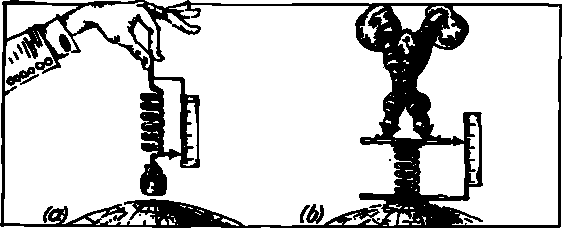
\includegraphics[width=\textwidth]{figures/fig-01-01.pdf}
\caption{Using extension and compression of springs for measuring weights.}
\label{fig-1.1}
\end{figure}
A calibrated spring can serve for measuring not only the force of the
Earth's attraction, i.e. weight, but also other forces. Such an
instrument is called a dynamometer, which means a measurer of
forces. You may have seen how a dynamometer is used for measuring a
person's muscular force. It is also convenient to measure the tractive
force of a motor by means of a stretching spring (\figr{fig-1.2}).
\begin{figure}[!ht]
\centering
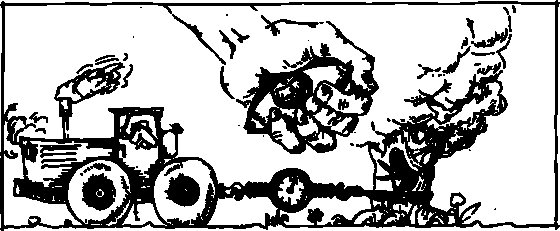
\includegraphics[width=\textwidth]{figures/fig-01-02.pdf}
\caption{A dynamometer is used to measure forces.}
\label{fig-1.2}
\end{figure}
The weight of a body is one of its very important properties. However,
the weight depends not only on the body itself. As a matter of fact,
the Earth attracts it.  And what if we were on the Moon? It is
obvious that its weight would be different -- about six times less, as
shown by computations. In fact, even on the Earth, weight is different
at various latitudes. At a pole, for example, a body weighs
0.5\% more than at the equator.

However, for all its changeability, weight possesses a remarkable
peculiarity -- the ratio of the weights of two -- bodies remains
unchanged under any conditions, as experiments have shown. If two
different loads stretch a spring identically at a pole, this identity
is completely preserved even at the equator.

In measuring weight by comparing it with the weight of a standard, we
find a new property of bodies, which is called \emph{mass}.

The physical meaning of this new concept -- mass -- is related in the most
intimate way to the identity in comparing weights which we have
just noted.

Unlike weight, mass is an invariant property of a body depending on
nothing except the given body.  

A comparison of weights, i.e. measurement of mass, is most
conveniently carried out with the aid of ordinary balance scales
(\figr{fig-1.3}). We say that the masses of
two bodies are equal if the balance scale on whose pans these bodies
are placed is in perfect equilibrium. If a load is in equilibrium on a
balance scale at the equator, and then the load and the weights are
transported to a pole, the load and the weights change their weight
identically. Weighing at the pole will therefore yield the same
result: the scale will remain balanced.

\begin{figure}
\centering
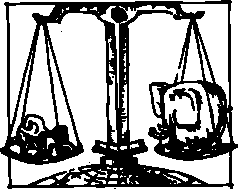
\includegraphics[width=0.45\textwidth]{figures/fig-01-03.pdf}
\caption{Measuring the mass with help of balance scales.}
\label{fig-1.3}
\end{figure}

We can even verify this state of affairs on the Moon. Since the
ratio of bodies' weights will not change there either, a load placed
on a scale will be balanced by the same weights there. The mass of a
body remains the same no matter where it is.


Units of mass and weight are related to the choice of a standard
weight. Just as in the case of the metre and the second, people tried
to find a natural standard of mass. The same commission used a
definite alloy to make a weight which balanced one cubic decimetre of
water at four degrees Centigrade\footnote{This temperature was not
  chosen by chance. Its significance lies in the fact that the volume
  of water changes with heating in a very peculiar manner, unlike most
  bodies. A body ordinarily expands when heated, but water contracts
  as its temperature rises from \SIrange{0}{4}{\degreeCelsius}, and
  only starts expanding after it gets above
  \SI{4}{\degreeCelsius}. Thus, \SI{4}{\degreeCelsius} is the
  temperature at which water stops to contract and begins to
  expand.}. This standard was called the \emph{kilogram}.


Later, however, it became clear that it isn't so easy to ``take'' one
cubic decimetre of water. Firstly, the decimetre, as a fraction of the
metre, changed along with the refinement of the metre's
standard. Secondly, what kind of water should we take? Chemically pure
water? Twice distilled? Without any trace of air? And what should be
done about admixtures of ``heavy water''? To top off all our
misfortunes, accuracy in measuring a volume is noticeably less than
that in weighing.


It again became necessary to reject a natural unit and accept a
specially made weight as the unit of mass. This weight is also kept in
Paris together with the standard for the metre.


One-thousandth and one-millionth of a kilogram -- the \emph{gram} and
the \emph{milligram} -- are widely used for measuring mass. The Tenth
and Eleventh General Conferences of Weights and Measures developed the
International System of Units (SI), which was then ratified by most
countries as national standards. The name ``kilogram'' (\si{\kg}) is
retained by mass in this system. Every force, including of course
weight, is measured in newtons (\si{\newton}) in this system. We shall
find out a bit later why this unit was given such a name and how it is
defined.

The new system will undoubtedly not be immediately and universally
applied, and so it is still helpful to recall that the kilogram of
mass (\si{kg}) and the kilogram of force (\si{\kgf}) are units of different
physical quantities, and it is impossible to perform arithmetical
operations on them.  Writing $\SI{5}{\kg} + \SI{2}{\kgf} = 7$ is just as meaningless as
adding metres to seconds. 

\section[The SI System and Standards of Measurement]{The International System of Units
and Standards of Measurement}
We began our discourse from the simplest things. For what can be
simpler than measuring distances, time intervals and mass? Indeed,
this was so in the early days of physics, but today the methods used
in measuring length, time and mass are so sophisticated that they
require a knowledge of all branches of physics. What we are going to
discuss now in more or less detail is studied in the fourth book,
\emph{Photons and Nuclei}. With this in mind, I suggest that if this is your
first book in physics, postpone reading this section until later.


The International System of Units, abbreviated SI from the French ``Le Syst\'eme International d'Unites'', was adopted in 1960. Slowly but surely it is gaining recognition. But even now when these lines are being written (on the threshold of 1977) the good ``old'' units of measurement are still in use. If you ask a car owner what engine his car has, his first reaction will be ``a 100 horse-power'' (just as, say, ten years ago) but not ``a 74 kilowatt''.  I believe that the SI system will become predominant only after two generations have passed and the books whose authors refuse to recognize it have gone out of print.  

The SI system is based on seven \emph{base} units: the metre, the kilogram, the second, the mole, the ampere, the kelvin and the candela.\footnote{In 2019 the SI system underwent a major change and both the base and the derived units were redefined in a fundamental manner. We will give the new definitions in the footnotes for each of the base units. -- Damitr}

Let us start with the first four. My purpose is to emphasize a
significant tendency of a general nature rather than to expound the
details of measuring the corresponding quantities. The tendency is to
discard material (i.e. man-made) standards and instead use natural
standards, that is, standards whose values do not depend on the
measuring devices and do not change with time, at least from the
viewpoint of today's physics.


We will begin with the metre. In the spectrum of a particular
isotope of Krypton, Kr$^{86}$, there is a sharp spectral line. By using
methods which we will discuss later it was established that each
spectral line is characterized by the initial and final energy
levels. The line we are interested in is the transition from the $5d_{5}$
level to the $2p_{10}$ level. Specifically, one metre is \num{1650763.73} wavelengths in vacuum of the radiation corresponding to the transition
between the levels $2p_{10}$ and $5d_{5}$ of the Krypton-$86$ atom. There is no
use in adding another significant digit to the above nine-digit
number, since the accuracy in measuring this wavelength is not more
than 4 parts in \num{d9}. We see that this definition is in no way
connected with a material standard. There is also no reason to believe
that the wavelength of a specific transition changes over the ages. So
we have achieved our goal.  


Well and good, my reader may say. But how does one calibrate an
ordinary yardstick with the aid of such a non-material standard?
Physicists know how to do this using interference methods, which we
will examine in the fourth book. 

There is every reason to assume that this definition will undergo a
change in the near future. The point is that using a laser beam (say,
of a helium-neon laser stabilized with iodine vapour) we can achieve
an accuracy of 1 part in \num{d11} or even 1 part in \num{d12}. It may
prove expedient to use another spectral line for the natural standard.

The definition of the second is quite similar. The transition used
is between two close energy levels of the Caesium-133 atom. The
inverse of the frequency of such a transition gives the time needed
for the completion of one vibration, the period. One second is taken
as \num{9192631770} such periods. Since these vibrations lie in the
microwave range, we can apply radio methods to divide the frequency
and thus calibrate any clock. The error is 1 second in \num{300000} years.


It was the dream of metrologists to use one energy transition for
defining the unit of length (expressed in a certain number of
wavelengths) and the unit of time (expressed in a certain number of
vibration periods).  

In 1973 scientists showed how this could be done. The measurements
were made using a helium-neon laser stabilized with methane. The
wavelength was 3.39 millimicrons, and the frequency was \num{88d-12}
cycles per second. The precision was so high that the product of these
two numbers gave the speed of light in vacuum as \num{299792458} metres
per second with an accuracy of 4 parts in \num{d9}. 
\label{sec-def}

In contrast to these brilliant achievements and still greater
prospects, the precision in measuring mass leaves much to be
desired. The ``material'' kilogram is still in use,
unfortunately. True, balances are constantly being perfected, but
still a precision of 1 part in \num{d9} is achieved only in rare cases and
only in comparing two masses.  The accuracy in measuring the mass of a
body in grams and in measuring the gravitational constant in the law
of universal gravitation still does not exceed 1 part in \num{d5}.

The Fourteenth General Conference of Weights and Measures (1971)
introduced into the SI system a new base unit of amount of substance,
the \emph{mole}. The introduction of the mole as an independent unit
of amount of substance is due to the new definition of the Avogadro
number.

It was agreed that the \emph{Avogadro number} was not just the number of
atoms in one gram-atom but the number of atoms in 12 grams of the
isotope of Carbon with mass number 12, that is C$^{12}$. If we denote the
number of atoms in 12 grams of C$^{12}$ as $N_{A}$, we define a mole as the
amount of substance that contains $N_{A}$ particles. The particle may be
an atom, a molecule, an ion, a radical, an electron, etc., or a
specified group of such entities.  

What makes it necessary to introduce not only a new base unit but a
new physical concept is the fact that we inadmissibly apply the
concept of mass to elementary particles, whereas mass is a quantity
measured with a beam balance.  

Today the amount of substance (the Avogadro number and, hence, atomic
mass) is determined with a lower accuracy than mass proper. But,
understandably, the accuracy of measuring the amount of substance
cannot exceed the accuracy of measuring mass.

My reader may think that the introduction of a new
unit is no more than a formality. However, the existence of two
concepts of mass is justified by the difference in precision of
measurement. If it ever proves possible to express the kilogram as a
multiple of the mass of an atom, the case will be reviewed and the
kilogram will become a quantity of the same type as the metre or
second.  

\section{Density}

What do we mean when we say: as heavy as lead and as light as a
feather? It is clear that a grain of lead will be light, while a
mountain of feathers has considerable mass. Those who use such
comparisons have in mind not the mass of a body but
the density of the material of which it consists.  

The mass of a unit volume of a body is called its \emph{density}. It
is evident that a grain of lead and a massive block of lead have the
same density.  

In denoting density, we usually indicate how many grams (\si{\gram}) a
cubic centimetre (\si{\cm^{3}}) of the body weighs -- after this
number we place the symbol \si{\gram\per\cm^{3}}. In order to
determine the density, the number of grams must be divided by the
number of cubic centimetres; the solidus in the symbol reminds us of
this.

Certain metals are among the heaviest materials -- Osmium whose
density is equal to \SI{22.5}{\gram\per\cm^{3}}, Iridium (22.4), Platinum (21.5),
Tungsten and Gold (19.3). The density of Iron is 7.88, that of Copper
8.93.  

The lightest metals are Magnesium (1.74), Beryllium (1.83) and
Aluminium (2.70). Still lighter bodies should be sought among organic
materials: various sorts of wood and plastic may have a density as low
as 0.4.  

It should be stipulated that we are dealing with continuous bodies. If
there are pores in a solid, it will of course be lighter. Porous
bodies -- cork, foam glass -- are frequently used in technology. The
density of foam glass may be less than 0.5, although the solid matter
from which it is made has a density greater than
\SI{1}{\gram\per\cm^{3}}. As all other bodies whose density is less
than \SI{1}{\gram\per\cm^{3}}, foam glass floats superbly on water.

The lightest liquid is liquid hydrogen; it can only be obtained at
extremely low temperatures. One cubic centimetre of liquid hydrogen
has a mass of \SI{0.07}{\gram}. Organic liquids -- alcohol, benzine,
kerosene -- do
not differ significantly from water in density. Mercury is very
heavy -- it has a density of \SI{13.6}{\gram\per\cm^{3}}. 

And how can the density of gases he characterized? For gases, as is
well known, occupy whatever volumes we let them. If we empty gas-bags
with the same mass of gas into vessels of different volumes, the gas
will always fill them up uniformly. How then can we speak of density?


We define the density of gases under so -- called normal conditions --
a temperature of \SI{0}{\celsius} and a pressure of 1 atm. The
density of air under normal conditions is equal to
\SI{0.00129}{\gram\per\cm^{3}}, of chlorine
\SI{0.00322}{\gram\per\cm^{3}}.  Gaseous hydrogen, just as the liquid
one, holds the record: the density of this lightest gas is equal to
\SI{0.00009}{\gram\per\cm^{3}}.

The next lightest gas is helium; it is twice as heavy as
hydrogen. Carbon dioxide is heavier than air by a factor of 1.5. In
Italy, near Naples, there is a famous ``canine cave''; carbon dioxide
continually exudes from its lower part, hangs low and slowly escapes
from the cave. A person can enter this cave without difficulty, but
such a stroll will end badly for a dog. Hence the cave's name.  

The density of gases is extremely sensitive to external
conditions-pressure and temperature. Without an indication of the
external conditions, the values of the density of gases have no
meaning. The densities of liquids and solids also depend on
temperature and pressure, but the dependence is considerably weaker.


%\newpage



\begin{center}
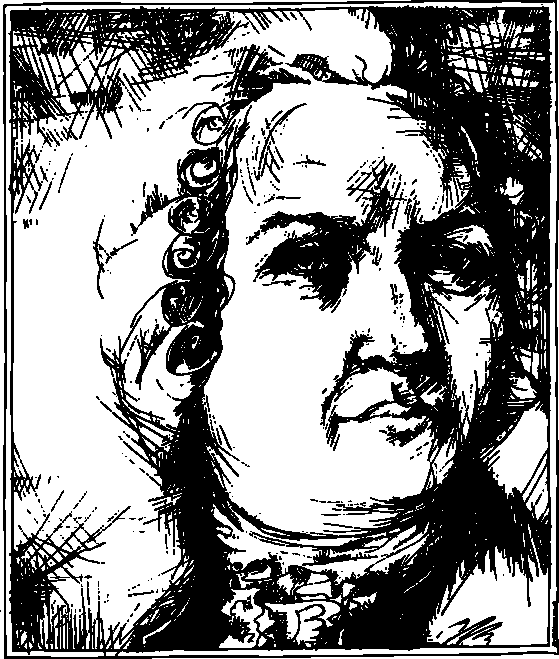
\includegraphics[width=0.8\textwidth]{figures/lomonosov.pdf}
\end{center}
{\small \textsf{{Mikhail Lomonosov [1711-1765]}} -- \textsf{\footnotesize an outstanding Russian scientist, the initiator of science in Russia, a great educator. In the field of physics, Lomonosov struggled resolutely against the notions widespread in the 18th century of electrical and thermal ``fluids'', upholding the molecular-kinetic theory of matter. Lomonosov was the first to experimentally prove the constancy of the mass of matter participating in chemical transformations. Lomonosov carried out extensive research in the field of atmospheric electricity and meteorology. He constructed a series of remarkable optical instruments and discovered the atmosphere on Venus. Lomonosov created the basis of scientific Russian; he succeeded in translating the basic physical and chemical terms from the Latin exceptionally well.}}


\section{The Law of Conservation of Mass}
If we dissolve some sugar in water, the mass of the solution will be
precisely equal to the sum of the masses of the sugar and the water.

This and an infinite number of similar experiments show that the mass
of a body is an invariable property.  No matter how the body is
crushed or dissolved, its mass remains fixed.  


The same also holds for arbitrary chemical transformations. Suppose
that coal burns up. It is possible to establish by means of careful
weighings that the mass of the coal and the oxygen from the air which
was used up during the burning will be exactly equal to the mass of
the end products of the combustion.  

The law of conservation of mass
was verified for the last time at the end of the 19th century, when
the technique of fine weighing had already been highly developed.
It turned out that mass does not even change by an insignificant
fraction of its value during the course of any chemical
transformation.  

Mass was considered to be invariable as far back as
Ancient Times. This law first underwent an actual experimental
verification in 1756. This was done by Mikhail Lomonosov, who proved
the conservation of mass during the sintering of metals by means of
experiments in 1756, and demonstrated the scientific significance the
law.  

Mass is the most important invariable characteristic of a
body. The majority of the properties of a body is, so to say, in the
hands of human beings. An iron bar that can be easily bent by hand can
be made hard and brittle by tempering it. With the aid of ultrasonic
waves, one can make a turbid solution transparent. Mechanical,
electrical and thermal properties can be changed by means of external
actions. If no matter is added to a body and not a single particle is
separated from it, it is impossible\footnote{The reader will later
  discover that there are certain limitations to this assertion.} to
change its mass, regardless of what external actions we resort to.



\section{Action and Reaction}
We frequently fail to notice that every action of a
force is accompanied by a reaction. If a valise is placed
on a bed with a spring mattress, the bed will sag. The fact
that the weight of the valise acts on the bed is obvious
to everyone. Sometimes, however, we forget that the bed
also exerts a force on the valise. As a matter of fact,
the valise lying on the bed does not fall; this means that
there is a force acting on it equal to the weight of the
valise and directed upwards.

Forces which are opposite in direction to gravity are
often called reactions of the support. The word ``reaction''
means ``counteraction''. The action of a table on a book
which is lying on it and the action of a bed on a valise
which has been placed upon it are reactions of the support.


As we have just said, the weight of a body can be determined with the
aid of a spring balance. The pressure of the body on the spring which
has been placed under it, or the force stretching the spring on which
the load has been suspended, is equal to the weight of the body. It is
obvious, however, that the contraction or tension of the spring can
just as well be used to obtain the value of the reaction of the
support.  

Thus, measuring the magnitude of some force by means of a
spring, we measure the value of not one but of two forces opposite in
direction. Spring balances measure the pressure exerted by the load on
the pan, and also the reaction of the support -- the action of the pan on
the load. Fastening a spring to a wall and pulling it by
hand, we can measure the force with which our hand pulls
the spring and, simultaneously, the force with which
the spring pulls our hand.

Therefore, forces possess a remarkable property: they
are always found in pairs and are, moreover, equal in
magnitude and opposite in direction. It is these two forces
which are usually called \emph{action and reaction}.


``Single'' forces do not exist in nature -- only mutual reactions
between bodies have a real existence; moreover, the forces of action
and reaction are invariably equal -- they are related to each other as
an object is related to its mirror image.  

One should not confuse
balancing forces with forces of action and reaction. We say that
forces are balanced if they are applied to a single body; thus, the
weight of a book lying on a table (the action of the Earth on the
book) is balanced by the reaction of the table (the action of the
table on the book).  


In contrast to the forces which arise in
balancing two interactions, the forces of action and reaction
characterize one interaction, for example, of a table with a book. The
action is ``table-book'' and the reaction is ``book-table''. These forces,
of course, are applied to different bodies.  

Let us try to clear up the following traditional misunderstanding:
``The horse is pulling the waggon, but the waggon is also pulling the
horse; why then do they move?'' First of all, we must recall that the
horse will not move the waggon if the road is slippery. Hence, in
order to explain the motion, we must take into account not one but two
interactions-not only ``waggon-horse'' but also ``horse-road''. The
motion will begin when the force of the interaction ``horse-road''
(the force with which the horse pushes off from the road) exceeds that
of the interaction ``waggon-horse'' (the force with which the waggon
pulls the horse). As for the forces ``waggon nulls horse'' and ``horse
pulls waggon'', they characterize one and the same interaction, and
will therefore be identical in magnitude when at rest and at any
instant during the course of the motion.
\section{How Velocities Are Added}

If I waited half an hour and then another hour, I would lose one and a
half hours of time all told. If I were given a rouble and then two
more, I would receive three roubles in all. If I bought
\SI{200}{\gram} of grapes and then another \SI{400}{\gram}, I would
have \SI{600}{\gram} of grapes. We say that time, mass and other
similar quantities are added arithmetically.

However, not every quantity can be added and subtracted so simply. If
I say that it is \SI{100}{\km} from Moscow to Kolomna and \SI{40}{\km}
from Kolomna to Kashira, it does not follow from this that Kashira is
located at a distance of \SI{140}{\km} from Moscow. Distances are not
added arithmetically.  

How else can quantities be added? We shall easily find the required
rule on the basis of our example. Let us draw three points on a piece
of paper indicating the relative locations of the three places of
interest to us (\figr{fig-1.4}). We can
construct a triangle with these three points as vertices. If two of
its sides are known, it is possible to find the third. For this,
however, we must know the angle between the two given segments.

%\addtocounter{figure}{-1}
\begin{figure}[!ht]
\centering
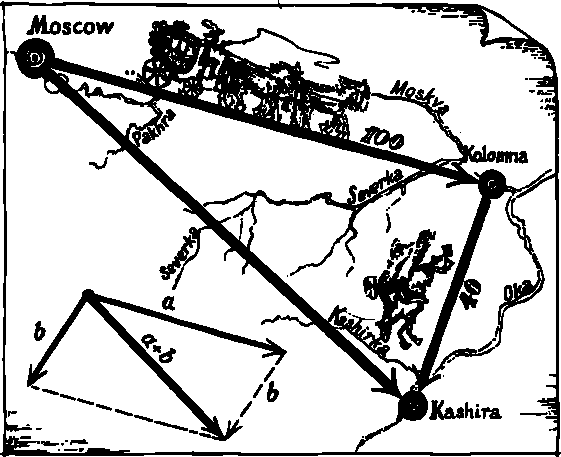
\includegraphics[width=\textwidth]{figures/fig-01-04.pdf}
\caption{Distances are not added artihmetically.}
\label{fig-1.4}
\end{figure}

The trip from Moscow to Kolomna can be represented by an arrow whose
direction shows where we are moving to. Such arrows are called
vectors. So the trip from Kolomna to Kashira is represented by
another vector.  

Now, how do we show the trip from Moscow to Kashira? With a vector, of
course. We will start this vector at the beginning of the first vector
and end it at the end of the second. The sought path will be the line
that completes the triangle.

The kind of addition just described is called geometrical and the
quantities which are added in this manner are called \emph{vectors}.

In order to distinguish the initial point of a segment from its end
point, we add an arrow to it. Such a segment -- a vector -- indicates a
length and a direction.  

This rule is also applied in adding several vectors.  Passing from the
first point to the second, from the second to the third, etc., we
cover a path which can be represented by a broken line. But it is
possible to go directly from the starting point to the terminal
point. This segment closing up the polygon will be precisely the
vector sum.  

A vector triangle also shows, of course, how to subtract one vector
from another. For this we draw them from one point. The vector drawn
from the end point of the second vector to the end point of the first
will be the vector difference.  

Besides the triangle rule, one may make use of the equivalent
parallelogram rule (\figr{fig-1.4} in the
lower left corner). This rule requires that we construct a
parallelogram on the vectors we are adding, and draw the diagonal from
the point of their intersection. It is clear from the figure that the
diagonal of the parallelogram is precisely the segment which closes up
the triangle. Hence, both rules are equally suitable.  

Vectors are used for describing not only displacements.  Vector
quantities are frequently found in physics.

Consider, for example, a velocity of motion. \emph{Velocity} is the
displacement during a unit of time. Since the displacement is a
vector, the velocity is also a vector, and it has the same
direction. In the course of motion along a curve, the direction of
displacement is changing all the time. How then can we answer the
question about the direction? A small segment of a curve has the same
direction as a tangent. Therefore, the displacement and velocity of a
body are directed along the tangent to the path of motion at each
given instant.  

In many cases one must add and subtract velocities
according to the rule for vectors. The need to add velocities arises
when a body participates simultaneously in two motions. Such cases are
not uncommon: a person walks inside a train and, in addition, moves
together with the train; a drop of water trickling down the window
pane of a train moves downwards under the action of its weight and
travels along with the train; the Earth moves around the Sun and
together with the Sun moves with respect to the other stars. In all
these and other similar cases, velocities are added in accordance with
the rule for adding vectors.

If both motions take place along a single line, then vector addition
reduces to ordinary addition when both motions have the same
direction, and to subtraction when they have opposite directions.  

But what if the motions take place at an angle? Then we turn to
geometrical addition.

If in crossing a swiftly flowing river you steer perpendicular to the
current, you will be carried downstream.  The boat participates in two
motions: across the river and along the river. The total velocity of
the boat is shown in \figr{fig-1.5}.  

\begin{figure}
\centering
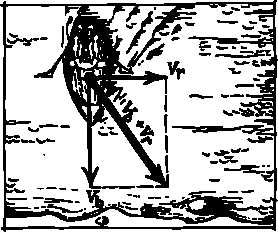
\includegraphics[width=0.5\textwidth]{figures/fig-01-05.pdf}
\caption{Adding vectors geometrically.}
\label{fig-1.5}
\end{figure}

Another example. What does the motion of a stream of raindrops look
like from the window of a train?  You have no doubt observed rain from
train windows. Even in windless weather it moves slantwise, as if a
wind blowing towards the train from ahead were deflecting it (
\figr{fig-1.6}).  

If the weather is windless, a raindrop falls vertically
downwards. But during the time the drop is falling near the window,
the train has travelled a fair distance leaving the vertical line of
fall behind; this is why the rain seems to be slanting.
\begin{figure}[!ht]
\centering
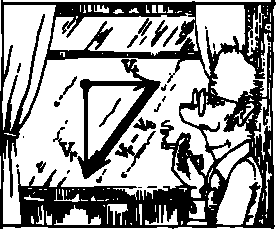
\includegraphics[width=0.5\textwidth]{figures/fig-01-06.pdf}
\caption{Why does the rain seem slanting from a moving train?}
\label{fig-1.6}
\end{figure}

If the velocity of the train is $\mathbf{v}_{t}$, and the velocity of
the raindrop is $\mathbf{v}_{r}$, then the velocity of its fall
relative to a passenger of the train is obtained by the vector
subtraction of $\mathbf{v}_{t}$ from $\mathbf{v}_{r}$.\footnote{Here
  and in what follows we shall use bold-face letters to denote
  vectors, i.e. characteristics for which not only magnitude but also
  direction is of significance.} The velocity triangle is shown in
\figr{fig-1.6}. The direction of the slanting
vector indicates the direction of the rain; now it is clear why we
see the rain slanting. The length of the slantwise arrow yields the
magnitude of this velocity in the chosen scale. The faster the train
goes and the slower the raindrop falls, the more the stream of
raindrops seems to slant.
\section{Force Is a Vector}
\emph{Force}, just as velocity, is a vector quantity. For it always
acts in a definite direction. Therefore, forces should also be added
according to the rules which we have just discussed.

We often observe examples in real life which illustrate the vector
addition of forces. A rope on which a package is hanging is shown in
 \figr{fig-1.7}. A person is pulling the package to one side with a
string. The rope is being stretched by the action of two forces: the
force of the weight of the package and the force that the person
exerts on it.
\begin{figure}[!ht]
\centering
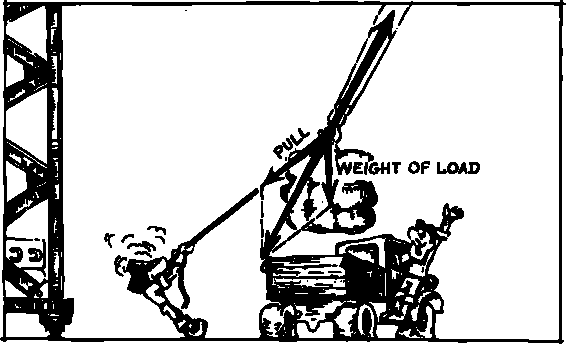
\includegraphics[width=\textwidth]{figures/fig-01-07.pdf}
\caption{Vector addition of forces.}
\label{fig-1.7}
\end{figure}
The rule of vector addition of forces allows us to determine the direction of the rope and compute the tension.
The package is at rest; hence, the sum of the forces acting
on it must be equal to zero. And we can also put it this
way -- the tension in the rope must be equal to the sum
of the weight of the package and the force pulling it to
one side with the aid of the string. The sum of these
forces yields the diagonal of a parallelogram which will
be directed along the rope (for otherwise it could not be
``annihilated'' by the tension in the rope). The length
of this arrow will represent the tension. The two forces
acting on the package could be replaced by such a force.
The vector sum of forces is therefore sometimes called
the resultant.

There very often arises a problem which is inverse to the addition of
forces. A lamp is suspended on two ropes.  In order to determine the
tension in the ropes, we must decompose the weight of the lamp along
these two directions.  
\begin{figure}[!ht]
\centering
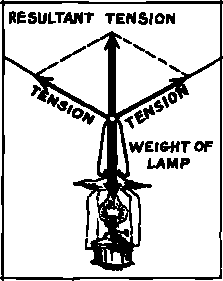
\includegraphics[width=0.4\textwidth]{figures/fig-01-08.pdf}
\caption{Determining the tension in the ropes.}
\label{fig-1.8}
\end{figure}

From the end point of the resultant vector
(\figr{fig-1.8}) we draw lines parallel to the ropes up to the points of
intersection. The parallelogram of forces is constructed.  Measuring
the lengths of the sides of the parallelogram, we find (in the same
scale in which the weight is represented) the magnitude of the
tension in the rope.  

Such a construction is called a decomposition of force. Every number can be represented in an infinite number of ways as the
sum of two or several numbers; the same thing can also be done with a
force vector: any force can be decomposed into two forces -- sides of
a parallelogram -- one of which can always be chosen arbitrarily. It
is also clear that to each vector there can be attached an arbitrary
polygon.

It is often convenient to decompose a force into two mutually
perpendicular forces -- one along a direction of interest to us and the other perpendicular to this direction. They are called the tangential and normal (perpendicular) components of force.  

The component of force in a particular direction, constructed by a
decomposition along the sides of a rectangle, is also called the
projection of the force in this direction.  
\begin{figure}
\centering
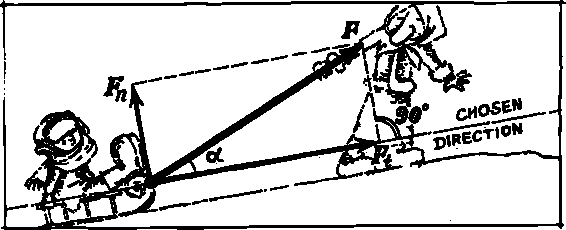
\includegraphics[width=\textwidth]{figures/fig-01-09.pdf}
\caption{Determining the tension in the ropes.}
\label{fig-1.9}
\end{figure}

It is clear that in \figr{fig-1.9}

\begin{equation*}%
F^{2} = F_{t}^{2} + F_{n}^{2} 
\end{equation*}

where $F_{t}$ and $F_{n}$ are the projections of
the force in the chosen direction and normal to it.  

Those who know
some trigonometry will establish without difficulty that 
\begin{equation*}%
F_{t} = F \cos \alpha
\end{equation*}

 where $\alpha$  is the angle between the force vector and the direction
onto which it is projected.  

A very curious example of the decomposition of forces is given by the
motion of a sailboat. How does it manage to sail against the wind? If
you ever watched a sailboat doing this, you might have noticed that it
zigzagged.  Sailors call such a motion tacking.  

\begin{figure}
\centering
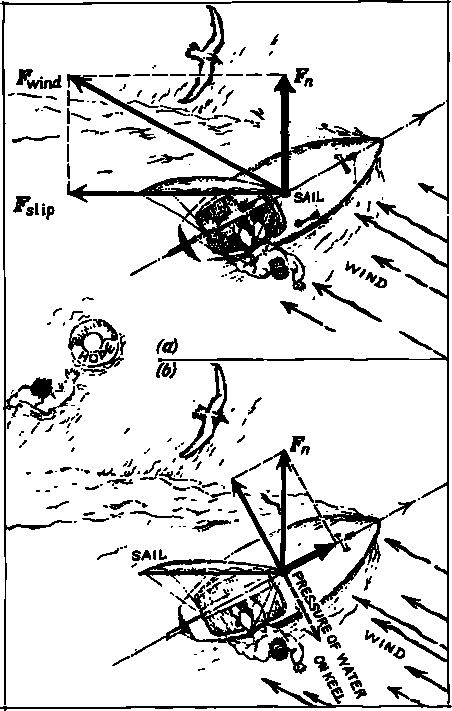
\includegraphics[width=0.9\textwidth]{figures/fig-01-10.pdf}
\caption{Analysing the motion of a sailboat.}
\label{fig-1.10}
\end{figure}


Of course, it is impossible to sail directly against the wind, but why
is it possible to sail against the wind at all, if only at an angle?

The possibility of beating against the wind is based on two
circumstances. The wind always pushes the sail at right angles to the latter's plane. Look at \figr{fig-1.10}~{\textcolor{black!70}{(a)}}: the force of wind is decomposed into two components -- one of them $F_{\textrm{slip}}$ makes the air slip past the sail and, hence, does not act on the sail, and the other -- the normal component-exerts pressure on the sail.

But why does the boat move not in the direction of the wind but
roughly in the direction of the bow?  This is explained by the fact that a movement of a boat across its keel line would meet with a very strong resistance on the part of the water. Therefore, in order for a boat to move forward, it is necessary that the force pressing on the sail should have a forward component along the keel line. This aspect is illustrated in \figr{fig-1.10}~{\textcolor{black!70}{(b)}}.

In order to find the force which drives the boat forward, we
must decompose the force of the wind a second time.  We have to
decompose the normal component along and across the keel line. It is
just the tangential component that drives the boat at an angle towards
the wind, and the normal component is balanced by the pressure of the
water exerted on the keel. The sail is set in such a way that its
plane bisects the angle between the direction of the path of the boat
and that of the wind.

\section{Inclined Plane}
\label{inc-plane}
It is more difficult to overcome a steep rise than a gradual one. It
is easier to roll a body up an inclined plane than to lift it
vertically. Why is this so, and how much easier is it? The law of the
addition of forces permits us to gain an understanding of these
matters.  

\begin{figure}[!ht]
\centering
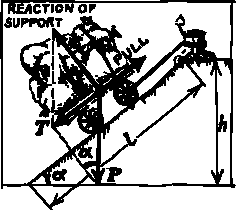
\includegraphics[width=0.6\textwidth]{figures/fig-01-11.pdf}
\caption{Analysing motion on an inclined plane.}
\label{fig-1.11}
\end{figure}

\figr{fig-1.11} depicts a waggon on wheels which is held on an
inclined plane by the tension in a string. Besides pull, two other
forces are acting on the waggon -- its weight and the force of the
reaction of the support which always acts along the normal to a
surface, regardless of whether the surface of the support is
horizontal or inclined.  

As has already been said, if a body rests
on a support, the latter counteracts the pressure Of, as we say,
creates the \emph{reaction force}.  

We want to know to what degree it is easier to pull a waggon up along
an inclined plane than to lift it vertically.  

We decompose the forces in such a way that one component is directed
along, and the other perpendicular to, the surface on which the body
is moving. In order for the body to be at rest on the inclined plane,
the tension in the string must balance only the tangential component.
As for the second component, it is balanced by the reaction of the
support.

We can find the force we are interested in, i.e. the tension $T$ in the
rope, either by means of a geometrical construction or with the aid of
trigonometry. The geometrical construction consists in dropping a
perpendicular from the end point of the weight vector $P$ to the plane.

One can find two similar triangles in the figure. The ratio of the
length $l$ of the inclined plane to its height $h$ is
equal to the ratio of the corresponding sides of the force
triangle. Thus,
\begin{equation*}
\frac{T}{P} = \frac{h}{l}
\end{equation*}

The less the plane is inclined (the smaller the value of
$h/l$), the easier it will be, of course, to pull the body
upwards.

And now, for those who are acquainted with trigonometry: since the
angle between the normal component of the weight and the weight vector is equal to the angle of inclination $\alpha$, of the plane (these are angles with mutually perpendicular sides), we have
\begin{equation*}
\frac{T}{P} = \sin \alpha \; \mathrm{and} \; T = P \sin \alpha
\end{equation*}
Therefore, it is $1/\sin \alpha$ times easier to wheel a
waggon up a plane with the angle of inclination $\alpha$ than to lift it vertically.  

It is helpful to memorize the values of the trigonometric functions for angles of \SIlist{30;45;60}{\degree}. Knowing these numbers for the sine ($\sin \ang{30} = 1/2; \; \sin \ang{45} = \sqrt{2}/2; \; \sin \ang{60} = \sqrt{3}/2$, we get a good idea of the amount of force saved by moving up an inclined plane.  

It is evident from our formulas that for a \ang{30} angle of
inclination, the force we exert will be half the weight of the body: $T = P/2$. For angles of \ang{45} and \ang{60}, we have to pull the rope with forces equal to about 0.7 and 0.9 of the weight of the waggon. As we see, such steeply inclined planes do not make our task much easier.
